\documentclass[journal]{IEEEtran}
\IEEEoverridecommandlockouts
\usepackage{cite}
\usepackage{amsmath,amssymb,amsfonts}
\usepackage{algorithm}
\usepackage{algpseudocode}
\usepackage{graphicx}
\usepackage{textcomp}
\usepackage{xcolor}
\usepackage{booktabs}
\usepackage{array}
\usepackage{multirow}
\usepackage{url}
\usepackage{tikz}
\usetikzlibrary{positioning,fit,arrows.meta,shapes.geometric,calc,backgrounds}
\usepackage{pgfplots}
\pgfplotsset{compat=1.16}
\definecolor{cblue}{RGB}{214,230,245}
\definecolor{cgreen}{RGB}{214,238,222}
\definecolor{corange}{RGB}{252,232,205}
\definecolor{cred}{RGB}{248,218,218}
\definecolor{cgray}{RGB}{238,238,240}
\definecolor{cblueD}{RGB}{40,100,170}
\definecolor{cgreenD}{RGB}{40,140,80}
\definecolor{corangeD}{RGB}{220,130,30}
\definecolor{credD}{RGB}{190,50,50}
\pgfplotsset{every axis/.append style={font=\scriptsize,tick label style={font=\tiny},label style={font=\scriptsize},legend style={font=\tiny,draw=none,fill=white,fill opacity=0.8,text opacity=1},grid=major,grid style={dotted,gray!50},width=\columnwidth,height=4.6cm}}
\newcommand{\E}{\mathbb{E}}
\newcommand{\Prob}{\mathbb{P}}
\def\BibTeX{{\rm B\kern-.05em{\sc i\kern-.025em b}\kern-.08em T\kern-.1em\lower.7ex\hbox{E}\kern-.125em X}}
\begin{document}
\title{Queueing and Branching-Process Models of Multi-Agent LLM Workflows: Latency, Failure, and Cost Prediction from Workflow Structure}
\author{\IEEEauthorblockN{Author Name}
\IEEEauthorblockA{\textit{Department, Institution}, City, Country (e-mail: email@institution.edu)}\thanks{A preliminary version of this work was presented at the authors' earlier conference paper; this journal version adds sub-agent trees, burst bracketing, service-time sensitivity, capacity planning, and an extended statistical evaluation.}}
\maketitle
\begin{abstract}
Multi-agent LLM systems are usually judged by task accuracy, while the dependence of their latency, failure rate, and cost on workflow structure is rarely modeled. This paper develops a semi-analytical performance model in which a task is a tree of agents, each agent executes a chain of steps, and each step issues a call to a shared G/G/$k$ LLM endpoint, spawns a random number of parallel tool calls that are joined, and may be retried after failure. Branching-process results give the number of agents and calls spawned and the criticality condition, an absorbing Markov chain gives success probability and cost per successful task, and Allen--Cunneen waiting-time approximations combined with numerically convolved response-time distributions give the full latency distribution, including a recursive fixed-point formulation for sub-agent trees. Validation against a discrete-event simulator with lognormal service times gives, for a single chain at utilization up to 0.8, errors of at most 2.3\%, 4.6\%, and 9.6\% in mean, p95, and p99 latency and success probability within 0.2 percentage points; for sub-agent trees with mean spawn 0.3--0.5 the worst-case errors at utilization 0.8 are 6.5\%, 9.3\%, and 14.1\%. The expected number of calls per successful task equals $\bar n/(1-p)$ regardless of the retry budget. Under bursty arrivals a Poisson model and a quasi-static Markov-modulated model bracketed the simulated latency in all 12 tested settings, while errors grow with service-time variability (mean latency overestimated by 31\% at a coefficient of variation of 2.5). Sizing a pool to a p99 target with a validation-derived 15\% margin met the target in the four tested pool sizes on average while admitting 13--26\% more load than a 0.7-utilization rule. All workloads are synthetic; calibration on measured traces remains future work.
\end{abstract}
\begin{IEEEkeywords}
multi-agent LLM systems, queueing networks, branching processes, fork-join queues, tail latency, capacity planning, performance modeling
\end{IEEEkeywords}

\section{Introduction}
Agentic LLM applications such as ReAct-style tool users, planner--worker hierarchies, and debate setups \cite{yao2023react,wu2023autogen,hong2024metagpt,du2023debate} are normally evaluated by task accuracy on a benchmark \cite{jimenez2024swebench,zhou2024webarena,liu2024agentbench}. Operators, however, must also answer questions of a different kind: how many LLM endpoint replicas keep p99 latency below a target, how much additional latency a wider tool fan-out costs, and how many retries a workflow can afford before the endpoint saturates. Kapoor et al. argue that agent benchmarks reward accuracy alone and call for evaluating cost and accuracy jointly \cite{kapoor2024agents}, and an analysis of more than 1{,}600 annotated execution traces from seven multi-agent frameworks catalogs 14 failure modes and finds that multi-agent designs often improve little over single-agent baselines \cite{cemri2025whyfail}. The resource side is substantial: in measurements of five agent designs, agents issued roughly nine times as many LLM calls as single-pass chain-of-thought prompting \cite{kim2025dynamic}.

Agent workloads differ from classical request streams in three ways. First, one LLM call triggers tool calls and, in hierarchical designs, further sub-agents, so the offered load is generated by a branching mechanism rather than by an exogenous Poisson stream. Second, parallel tool calls and sub-agents must be joined before the parent proceeds, and fan-out of this kind is a known amplifier of tail latency \cite{dean2013tail} whose synchronization makes analysis hard \cite{nelson1988forkjoin}. Third, failures are retried, so the failure probability of a step changes both the success probability and the load placed on shared endpoints.

This paper builds a model that connects these effects and tests it against a simulator. Relative to the preliminary conference version, the journal version adds a recursive model of sub-agent trees, an empirical bracketing treatment of bursty arrivals, a sensitivity study of service-time variability, a capacity-planning procedure with validation, a statistical treatment with confidence intervals, and a discussion of deployment and reproducibility. The contributions are as follows.
\begin{itemize}
\item A workflow model that couples a Galton--Watson spawning mechanism, an absorbing Markov chain for retries, and a two-station queueing network with fork-join synchronization (Section~\ref{sec:method}).
\item Closed-form results for total calls spawned, extinction probability, success probability, and cost per successful task, including the observation that cost per success is independent of the retry budget for geometric workflow length (Section~\ref{sec:math}).
\item A semi-analytical algorithm that returns the full latency distribution, and therefore p95 and p99, from structural parameters (Algorithm~\ref{alg:predict}), and its extension to recursive sub-agent trees through a fixed-point equation (Section~\ref{sec:tree}).
\item A burst-bracketing result and a margin-based sizing rule for p99 targets, each validated against simulation (Sections~\ref{sec:burst} and~\ref{sec:plan}).
\item A validation study with ablations, bottleneck analysis, service-time sensitivity, and an explicit account of where the model fails (Sections~\ref{sec:results}--\ref{sec:limits}).
\end{itemize}
An important scope note applies throughout: the service-time and structural parameters used here are assumed values, not measurements from a deployed agent framework, so the validation shows that the analytical model is consistent with its own simulated assumptions and quantifies approximation error, not that it fits real agent traces.

\section{Related Work}
\textbf{Agent frameworks and tool use.} ReAct interleaves reasoning and tool actions \cite{yao2023react}, AutoGen, MetaGPT, CAMEL, and AgentVerse organize multiple conversing agents \cite{wu2023autogen,hong2024metagpt,li2023camel,chen2024agentverse}, and generative agents simulate long-running behavior \cite{park2023generative}. Surveys catalog these designs \cite{wang2024survey}. Tool use and planning are studied in \cite{schick2023toolformer,shinn2023reflexion,wei2022cot}, and LLMCompiler explicitly parallelizes function calls \cite{kim2024llmcompiler}, which creates the fork-join structure analyzed here.

\textbf{LLM serving.} Serving systems optimize batching, memory, and scheduling at the endpoint level \cite{kwon2023vllm,yu2022orca,agrawal2024sarathi,zhong2024distserve,patel2024splitwise}, and energy-aware cluster design has been studied in \cite{stojkovic2025dynamollm}. Parrot moves one level up and schedules whole LLM applications with dependencies between calls \cite{lin2024parrot}. These works optimize or measure systems; they do not provide a predictive model linking workflow structure to latency distributions.

\textbf{Queueing and branching theory.} Jackson networks and heavy-traffic approximations \cite{jackson1957networks,halfin1981heavy,kingman1961heavy}, the GI/G/$m$ approximations of Whitt \cite{whitt1993approx}, and textbook treatments \cite{harchol2013performance} supply the single-station tools we use. Fork-join queues are analytically hard in general \cite{baccelli1989acyclic,nelson1988forkjoin}, and microservice benchmarks show that such dependencies drive tail latency in practice \cite{gan2019deathstar}. Branching processes \cite{harris1963branching,athreya1972branching} describe spawning, Hawkes and Markov-modulated processes describe self-exciting or bursty arrivals \cite{hawkes1971spectra,bacry2015hawkes,fischer1993mmpp}, and likelihood-based selection with AIC \cite{akaike1974aic} and heavy-tail testing \cite{clauset2009power,mitzenmacher2004lognormal} supports parameter estimation from traces.

\textbf{Analytical models of LLM serving and agents.} A queueing literature on LLM systems is emerging. Mitzenmacher and Shahout survey how queueing with predicted service times applies to LLM inference and pose open problems tied to variable run times and key-value memory limits \cite{mitzenmacher2025queueing}. Dai et al. model agent workloads as multi-class networks of batch-service LLM servers with DAG and fork-join routing and prove that work-conserving scheduling is throughput-optimal; their analysis targets stability, and the authors leave latency (service-level) attainment to future work beyond preliminary measurements \cite{dai2025throughput}. Ramani and Tantawi build an approximate Markovian model of a single LLM server that predicts mean time to first token and inter-token latency, and they report average errors of about 5--16\% against measurements on one GPU type \cite{ramani2026approximate}. At the workflow level, Yang and Zhu optimize latency, reliability, and cost of agentic workflows; they compose parallel branches through the expected maximum of branch latencies but work with expected latency and do not model contention for shared capacity \cite{yang2026reliable}. Systems work such as Autellix exploits program-level dependencies to schedule agent calls and reports 4--15$\times$ throughput gains over vLLM at equal latency \cite{luo2025autellix}, which shows that cross-call structure matters in practice but does not yield a predictive model.

\textbf{Measured agent workloads.} Recent measurement studies supply the quantities such models need. A trace of about 4{,}300 coding-agent sessions reports on average 8.8 LLM calls and 10.8 tool calls per request, and tool calls longer than one minute make up about 4\% of calls but 85\% of tool time \cite{zhu2026tracelab}. A ten-application benchmark finds that non-LLM components dominate latency in five of the ten applications \cite{chang2026agentic}, and production LLM traffic exhibits request burstiness that varies across services and models \cite{wang2024burstgpt}. All four studies are preprints at the time of writing.

\begin{table*}[t]
\caption{Comparison with the closest analytical work identified (\checkmark: modeled; --: not modeled in the parts of the paper we read). Entries are based on the cited papers' abstracts and the sections we accessed}
\label{tab:gap}
\centering
\footnotesize
\setlength{\tabcolsep}{4pt}
\begin{tabular}{lcccccc}
\toprule
Work & Shared pools & Fork-join & Retries on failure & Spawning & Latency output & Validation \\
\midrule
Dai et al. \cite{dai2025throughput} & \checkmark & \checkmark & -- & -- & stability only & theory, measured systems \\
Ramani, Tantawi \cite{ramani2026approximate} & one server & -- & -- & -- & means & GPU measurements \\
Yang, Zhu \cite{yang2026reliable} & -- & expected max & -- & -- & means & numerical \\
This paper & \checkmark & \checkmark & \checkmark & \checkmark & distribution & simulation only \\
\bottomrule
\end{tabular}
\end{table*}

\textbf{Gap.} Table~\ref{tab:gap} summarizes the closest work we identified. Among the studies we reviewed, none combines shared-pool queueing, fork-join, failure-driven retries, and spawning in a model that predicts latency percentiles and cost per successful task from structural parameters. Each ingredient appears separately: fork-join stability in \cite{dai2025throughput}, single-server latency prediction with hardware validation in \cite{ramani2026approximate}, and parallel composition with reliability and cost in \cite{yang2026reliable}. The contribution of this paper is their combination and an explicit account of its approximation error; unlike \cite{ramani2026approximate}, our validation is against simulation rather than measurement. Our search was bounded (Section~\ref{sec:limits}), so this is a statement about the literature we found, not a claim of priority.

\textbf{Capacity planning.} Classical capacity planning combines utilization limits with queueing approximations \cite{lazowska1984quantitative,bolch2006queueing}. Utilization thresholds are simple but ignore workflow structure, which in agent systems determines both the load multiplier (spawned calls and retries) and the tail (fork-join). Section~\ref{sec:plan} compares a threshold rule with model-based sizing.


\section{Proposed Framework}\label{sec:method}
\subsection{Workflow Model}
A task arrives at rate $\lambda$ and consists of $N$ sequential steps, where $N$ is geometric on $\{1,2,\dots\}$ with mean $\bar n=1/q$. Each step attempt (i) submits one call to the LLM pool with $k_L$ servers and service time $S_L$, (ii) on completion spawns $K$ parallel tool calls to a tool pool with $k_T$ servers and service time $S_T$, and (iii) joins when all tool calls return. The attempt then fails independently with probability $p$. A failed attempt is retried until $R$ retries have been used, after which the task fails. Fan-out $K$ is either fixed or Poisson with mean $\mu_K$, the latter being a one-generation Galton--Watson offspring law. Both service times are lognormal, a standard heavy-tailed model \cite{mitzenmacher2004lognormal}; this is an assumption, and measured tool latencies can be considerably heavier-tailed (Section~\ref{sec:discuss}). Hierarchical designs are modeled by letting a successful chain delegate to a random number of sub-agents, each running the same kind of chain, which the parent must join (Section~\ref{sec:tree}).

The model rests on four approximations: the superposition of many concurrent tasks makes arrivals to each pool close to Poisson; each pool behaves as a G/G/$k$ queue approximated by Allen--Cunneen; the response times of the $K$ parallel tool calls are independent given the pool state; and step times are independent across steps and attempts. Where these fail is the subject of Sections~\ref{sec:burst} and~\ref{sec:limits}.

\subsection{Structural Profiles}
We evaluate three illustrative profiles that mimic the structure, not the content, of common designs: P1 is deep and narrow (ReAct-like, $\bar n{=}8$, $\mu_K{=}1$), P2 is wide and shallow (planner--worker-like, $\bar n{=}4$, $K{=}6$), and P3 is balanced ($\bar n{=}5$, $\mu_K{=}2$).

\section{System Architecture}\label{sec:arch}
Fig.~\ref{fig:overview} shows the modeled system. Tasks enter through an arrival process, the workflow engine executes one step attempt at a time, and each attempt traverses the LLM pool, a fork to the tool pool, and a join. The retry controller closes the loop on failure, and in hierarchical designs a successful chain delegates to sub-agents as in Fig.~\ref{fig:tree}. Fig.~\ref{fig:pipeline} shows the evaluation pipeline: a shared configuration feeds both the analytical model and the discrete-event simulator, and their outputs are compared by relative error.
\begin{figure*}[t]
\centering
\resizebox{0.92\textwidth}{!}{%
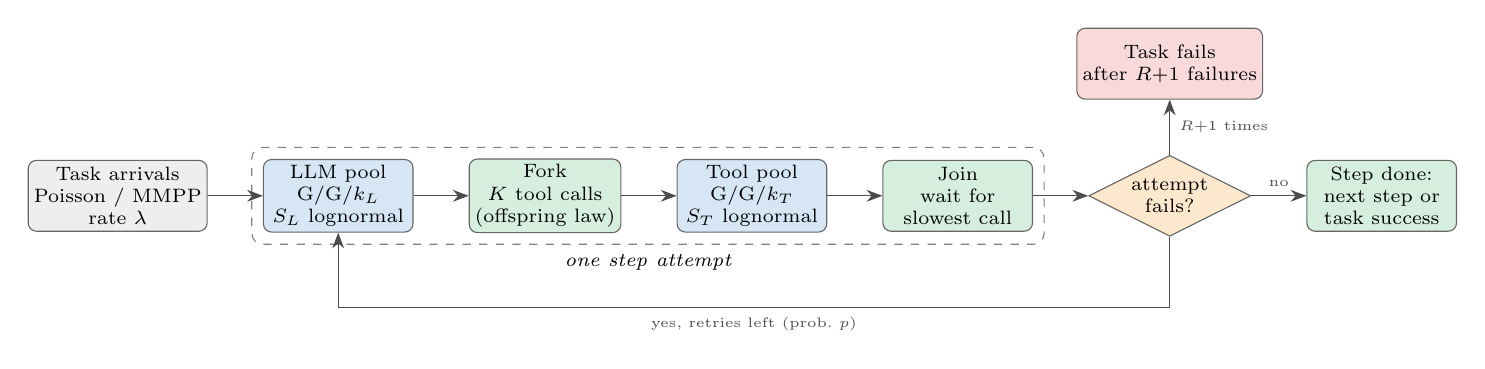
\begin{tikzpicture}[font=\scriptsize,node distance=6mm and 7mm,
box/.style={draw=black!60,rounded corners=3pt,fill=cblue,minimum height=9mm,minimum width=19mm,align=center,inner sep=2pt},
dec/.style={draw=black!60,diamond,aspect=2,fill=corange,align=center,inner sep=1pt},
every edge/.style={draw,-{Stealth[length=2mm]},black!70}]
\node[box,fill=cgray] (arr) {Task arrivals\\Poisson / MMPP\\rate $\lambda$};
\node[box,right=of arr] (llm) {LLM pool\\G/G/$k_L$\\$S_L$ lognormal};
\node[box,right=of llm,fill=cgreen] (fork) {Fork\\$K$ tool calls\\(offspring law)};
\node[box,right=of fork] (tool) {Tool pool\\G/G/$k_T$\\$S_T$ lognormal};
\node[box,right=of tool,fill=cgreen] (join) {Join\\wait for\\slowest call};
\node[dec,right=7mm of join] (dec) {attempt\\fails?};
\node[box,right=7mm of dec,fill=cgreen] (next) {Step done:\\next step or\\task success};
\node[box,above=7mm of dec,fill=cred] (fail) {Task fails\\after $R{+}1$ failures};
\node[draw=black!50,dashed,rounded corners=4pt,fit=(llm)(fork)(tool)(join),inner sep=4pt,label={[font=\scriptsize\itshape]below:one step attempt}] (att) {};
\draw (arr) edge (llm); \draw (llm) edge (fork); \draw (fork) edge (tool); \draw (tool) edge (join);
\draw (join) edge (dec); \draw (dec) edge node[above,font=\tiny]{no} (next);
\draw (dec) edge node[right,font=\tiny]{$R{+}1$ times} (fail);
\draw[-{Stealth[length=2mm]},black!70] (dec.south) -- ++(0,-9mm) -| node[pos=0.25,below,font=\tiny]{yes, retries left (prob.\ $p$)} (llm.south);
\end{tikzpicture}}
\caption{Modeled system. Each step attempt traverses the shared LLM pool, a fork into $K$ parallel tool calls, the tool pool, and a join; failed attempts return to the LLM pool until the retry budget is exhausted.}
\label{fig:overview}
\end{figure*}
\begin{figure}[t]
\centering
\resizebox{\columnwidth}{!}{%
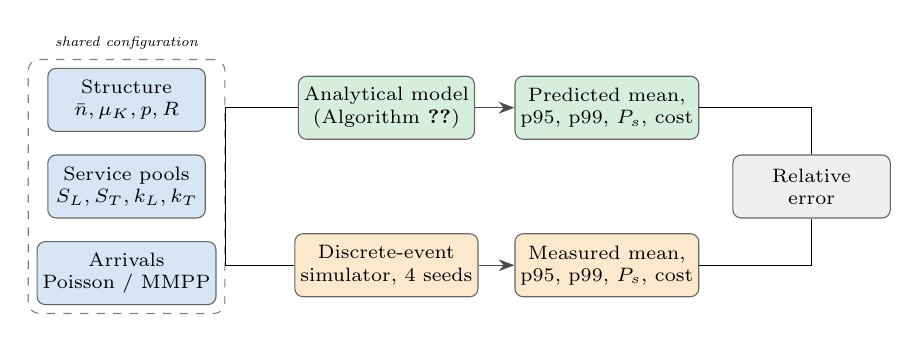
\begin{tikzpicture}[font=\scriptsize,
box/.style={draw=black!60,rounded corners=3pt,fill=cblue,minimum height=8mm,minimum width=20mm,align=center,inner sep=2pt},
every edge/.style={draw,-{Stealth[length=2mm]},black!70}]
\node[box] (in1) at (0,1.1) {Structure\\$\bar n,\mu_K,p,R$};
\node[box] (in2) at (0,0) {Service pools\\$S_L,S_T,k_L,k_T$};
\node[box] (in3) at (0,-1.1) {Arrivals\\Poisson / MMPP};
\node[draw=black!50,dashed,rounded corners=4pt,fit=(in1)(in2)(in3),inner sep=3pt,label={[font=\tiny\itshape]above:shared configuration}] (cfg) {};
\node[box,fill=cgreen] (mod) at (3.3,1.0) {Analytical model\\(Algorithm~\ref{alg:predict})};
\node[box,fill=corange] (des) at (3.3,-1.0) {Discrete-event\\simulator, 4 seeds};
\node[box,fill=cgreen] (o1) at (6.1,1.0) {Predicted mean,\\p95, p99, $P_s$, cost};
\node[box,fill=corange] (o2) at (6.1,-1.0) {Measured mean,\\p95, p99, $P_s$, cost};
\node[box,fill=cgray] (err) at (8.7,0) {Relative\\error};
\draw (cfg.east) |- (mod.west); \draw (cfg.east) |- (des.west);
\draw (mod) edge (o1); \draw (des) edge (o2); \draw (o1.east) -| (err.north); \draw (o2.east) -| (err.south);
\end{tikzpicture}}
\caption{Evaluation pipeline. The same configuration drives the analytical model and the simulator, and the validation metric is the relative error of each output.}
\label{fig:pipeline}
\end{figure}

\begin{figure}[t]
\centering
\resizebox{\columnwidth}{!}{%
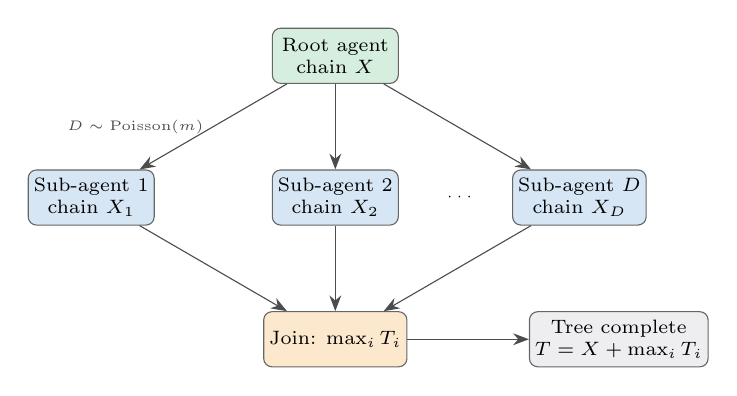
\begin{tikzpicture}[font=\scriptsize,
box/.style={draw=black!60,rounded corners=3pt,fill=cblue,minimum height=7mm,minimum width=16mm,align=center,inner sep=2pt},
every edge/.style={draw,-{Stealth[length=2mm]},black!70}]
\node[box,fill=cgreen] (root) at (0,0) {Root agent\\chain $X$};
\node[box] (a1) at (-3.1,-1.8) {Sub-agent 1\\chain $X_1$};
\node[box] (a2) at (0,-1.8) {Sub-agent 2\\chain $X_2$};
\node[box] (a3) at (3.1,-1.8) {Sub-agent $D$\\chain $X_D$};
\node[box,fill=corange] (j) at (0,-3.6) {Join: $\max_i T_i$};
\node[box,fill=cgray] (done) at (3.6,-3.6) {Tree complete\\$T=X+\max_i T_i$};
\draw (root) edge node[left,font=\tiny,pos=0.5]{$D\sim\mathrm{Poisson}(m)$} (a1); \draw (root) edge (a2); \draw (root) edge (a3);
\draw (a1) edge (j); \draw (a2) edge (j); \draw (a3) edge (j); \draw (j) edge (done);
\node[font=\tiny] at (1.6,-1.8) {$\cdots$};
\end{tikzpicture}}
\caption{Sub-agent tree. A root agent completes its chain, delegates to $D$ sub-agents that each run a chain (and may delegate further), and completes when all sub-agents have completed.}
\label{fig:tree}
\end{figure}

\section{Mathematical Model}\label{sec:math}
\subsection{Branching and Call Volume}\label{sec:branching}
Let the number of children per call have mean $m$ and variance $\sigma^2$. For $m<1$ the total progeny $Z$ of a tree rooted at one call satisfies
\begin{equation}\E[Z]=\frac{1}{1-m}\label{eq:meanZ}\end{equation}
\begin{equation}\mathrm{Var}[Z]=\frac{\sigma^2}{(1-m)^3}\label{eq:varZ}\end{equation}
\cite{harris1963branching,athreya1972branching}. For $m>1$ the tree dies out with probability $\xi$, the smallest root in $[0,1]$ of
\begin{equation}\xi=G(\xi),\qquad G(z)=\E[z^{K}]\label{eq:extinct}\end{equation}
and for Poisson offspring the total progeny follows the Borel law
\begin{equation}\Prob(Z=n)=\frac{e^{-mn}(mn)^{n-1}}{n!}.\label{eq:borel}\end{equation}
Estimating criticality from $n$ observed offspring counts gives, by the delta method, a relative standard error on $\E[Z]$ of approximately
\begin{equation}\frac{\mathrm{se}(\hat Z)}{\E[Z]}\approx\frac{\sigma}{\sqrt n\,(1-m)}\label{eq:est}\end{equation}
which diverges as $m\to1$ and explains why trace-based criticality tests are fragile near the boundary (Section~\ref{sec:results}).

\subsection{Retries and Cost}
With per-attempt failure probability $p$ and at most $R$ retries, a step succeeds with probability $s$ and consumes on average $a$ attempts,
\begin{equation}s=1-p^{R+1},\qquad a=\frac{1-p^{R+1}}{1-p}.\label{eq:succ}\end{equation}
Let $\nu$ be the expected number of started steps. Since a started step is followed by another with probability $(1-q)s$,
\begin{equation}\nu=\frac{1}{1-(1-q)s},\qquad P_s=q\,s\,\nu.\label{eq:nu}\end{equation}
The expected LLM calls per task is $c_L=\nu a$, and dividing by $P_s$ gives
\begin{equation}C_s=\frac{c_L}{P_s}=\frac{a}{q\,s}=\frac{\bar n}{1-p}\label{eq:cost}\end{equation}
which does not depend on $R$: extra retries raise $P_s$ and the load per started step in exactly compensating proportions. Retries therefore buy reliability, not cost savings, and under a constant per-call energy $\epsilon$ the energy per successful task is $\epsilon\,\bar n/(1-p)$.

\subsection{Load and Stability}
The offered loads on the two pools are
\begin{equation}\rho_L=\frac{\lambda\,c_L\,\E[S_L]}{k_L},\qquad \rho_T=\frac{\lambda\,c_L\,\E[K]\,\E[S_T]}{k_T}\label{eq:load}\end{equation}
and the system is stable for arrival rates below
\begin{equation}\lambda^\ast=\min\left\{\frac{k_L}{c_L\E[S_L]},\;\frac{k_T}{c_L\E[K]\E[S_T]}\right\}\label{eq:lamstar}\end{equation}
so the pool attaining the minimum is the bottleneck.

\subsection{Pool Response Time}
For a pool with $k$ servers and offered load $\alpha=\lambda\E[S]$, the Erlang-C probability of waiting is
\begin{equation}C(k,\alpha)=\frac{\alpha^k/\left(k!\,(1-\alpha/k)\right)}{\sum_{j=0}^{k-1}\alpha^j/j!+\alpha^k/\left(k!\,(1-\alpha/k)\right)}\label{eq:erlang}\end{equation}
and the two-moment approximation commonly attributed to Allen and Cunneen scales the M/M/$k$ mean wait by the squared coefficients of variation of arrivals and service; for $k=1$ it has the form of Kingman's heavy-traffic approximation \cite{kingman1961heavy}, and Whitt develops and evaluates two-moment approximations of this kind for GI/G/$m$ queues \cite{whitt1993approx},
\begin{equation}\E[W]\approx\frac{C(k,\alpha)}{k/\E[S]-\lambda}\cdot\frac{c_a^2+c_s^2}{2}.\label{eq:ac}\end{equation}
We model the wait as zero with probability $1-C$ and exponential otherwise, with the mean matched to Eq.~(\ref{eq:ac}),
\begin{equation}F_W(t)=1-C\,e^{-tC/\E[W]}\label{eq:wait}\end{equation}
and obtain the response-time distribution by convolution,
\begin{equation}F_R=F_W\ast F_S.\label{eq:resp}\end{equation}

\subsection{Fork-Join and End-to-End Latency}
Treating the $K$ tool responses as independent, the join time has CDF $F_R^{T}(t)^{K}$ for fixed $K$ and $\exp\{\mu_K(F_R^{T}(t)-1)\}$ for Poisson $K$, in general
\begin{equation}F_J(t)=G\!\left(F_R^{T}(t)\right).\label{eq:fj}\end{equation}
Approximating a join by the maximum of independent task response times is a standard device in fork/join analysis, and Thomasian's survey reports it as an estimate and an upper bound when the servers also process other requests \cite{thomasian2014forkjoin}; in our model the $K$ siblings enter the same pool at the same instant, a setting that guarantee does not cover (Section~\ref{sec:results}). The duration of one attempt is the sum of an LLM response and a join time, so its density is
\begin{equation}f_A=f_R^{L}\ast f_J.\label{eq:att}\end{equation}
Given that a step succeeds, the number of attempts is $i\in\{1,\dots,R+1\}$ with probability $w_i\propto p^{i-1}(1-p)$, hence
\begin{equation}f_{\mathrm{step}}=\sum_{i=1}^{R+1}w_i\,f_A^{\ast i}.\label{eq:step}\end{equation}
Conditioning a task on success tilts the step count to $\pi_n\propto q(1-q)^{n-1}s^n$, and
\begin{equation}f_{\mathrm{task}}=\sum_{n\ge1}\pi_n\,f_{\mathrm{step}}^{\ast n}\label{eq:task}\end{equation}
\begin{equation}t_\alpha=\inf\{t:F_{\mathrm{task}}(t)\ge\alpha\}\label{eq:quant}\end{equation}
where Eq.~(\ref{eq:quant}) yields p95 and p99 for $\alpha=0.95,0.99$. Algorithm~\ref{alg:predict} summarizes the computation; densities are discretized on a grid of $G=30{,}000$ points with $\Delta t=0.02$\,s and convolutions use the FFT, so the cost is $O\big((n_{\max}+R)\,G\log G\big)$ and does not depend on $\lambda$.
\begin{algorithm}[t]
\caption{Semi-analytical latency prediction}\label{alg:predict}
\begin{algorithmic}[1]
\Require $\lambda,\bar n,\mu_K\text{ or }K,p,R,(k_L,S_L),(k_T,S_T),c_a^2$
\State Compute $s,a,\nu,P_s,c_L$ by Eqs.~(\ref{eq:succ}), (\ref{eq:nu}); compute $\rho_L,\rho_T$ by Eq.~(\ref{eq:load})
\If{$\rho_L\ge1$ \textbf{or} $\rho_T\ge1$} \State \Return unstable \EndIf
\State $f_R^{L}\gets$ Eqs.~(\ref{eq:erlang})--(\ref{eq:resp}) with $(\lambda c_L,k_L,S_L)$
\State $f_R^{T}\gets$ Eqs.~(\ref{eq:erlang})--(\ref{eq:resp}) with $(\lambda c_L\E[K],k_T,S_T)$
\State $F_J\gets$ Eq.~(\ref{eq:fj}); $f_A\gets$ Eq.~(\ref{eq:att}); $f_{\mathrm{step}}\gets$ Eq.~(\ref{eq:step})
\State $f_{\mathrm{task}}\gets$ Eq.~(\ref{eq:task}) truncated at $n_{\max}=80$
\State \Return $P_s$, $\E[T]$, $t_{0.95}$, $t_{0.99}$ by Eq.~(\ref{eq:quant})
\end{algorithmic}
\end{algorithm}

\subsection{Sub-Agent Trees}\label{sec:tree}
Let each agent, after completing its chain successfully, delegate to $D\sim\mathrm{Poisson}(m)$ sub-agents that run the same kind of chain, and let the agent complete when all sub-agents have completed. A tree fails if any chain exhausts its retries. With chain success probability $P_s$ from Eq.~(\ref{eq:nu}), the number of agents started per tree is
\begin{equation}M=\frac{1}{1-mP_s}\label{eq:agents}\end{equation}
and the tree success probability $S$ is the smallest root of
\begin{equation}S=P_s\exp\{m(S-1)\}.\label{eq:treesucc}\end{equation}
Conditioned on tree success, the number of sub-agents is Poisson with mean $mS$, because thinning by the success event rescales the Poisson mean. Writing $F_T$ for the latency CDF of successful trees and $f_X$ for the density of a successful chain given by Eq.~(\ref{eq:task}), the tree latency $T=X+\max_{i\le D}T_i$ satisfies, under independence of sub-trees,
\begin{equation}F_T=f_X\ast\frac{d}{dt}\exp\{mS\,(F_T-1)\}\label{eq:treeF}\end{equation}
which we solve by fixed-point iteration on the discretization grid starting from $F_T=\int f_X$. Because tree arrivals at the pools are scaled by $M$ in expectation, the LLM utilization becomes
\begin{equation}\rho_L=\frac{\lambda\,M\,c_L\,\E[S_L]}{k_L}\label{eq:treeload}\end{equation}
and the chain densities in Eq.~(\ref{eq:treeF}) are computed at the inflated rates of Eq.~(\ref{eq:treeload}). The iteration converged in at most 20 steps in our experiments. Delegation also correlates arrivals, since $D$ sub-agents start simultaneously, which the model ignores.

\subsection{Bursty Arrivals: Bracketing}\label{sec:burst}
Stationary G/G/$k$ approximations fail under long bursts (Section~\ref{sec:limits}), and burstiness is documented in production LLM traffic \cite{wang2024burstgpt}. For a two-state MMPP with mean rate $\lambda$, high-state fraction $f$, and burst factor $\beta$, the low- and high-state rates are
\begin{equation}r_0=\frac{\lambda}{1-f+\beta f},\qquad r_1=\beta r_0\label{eq:rates}\end{equation}
and tasks arrive in the high state with probability $w_1=f\beta/(1-f+\beta f)$. The rates enter through Eq.~(\\ref{eq:rates}); we define two predictors. The Poisson predictor ignores burstiness and uses $\lambda$. The quasi-static predictor treats each state as stationary and mixes the corresponding latency distributions,
\begin{equation}F_{\mathrm{QS}}=(1-w_1)\,F_{\mathrm{task}}(r_0)+w_1\,F_{\mathrm{task}}(r_1)\label{eq:qs}\end{equation}
and is undefined if $\rho_L(r_1)\ge1$. The Poisson predictor ignores state changes and is expected to underestimate; the quasi-static predictor ignores the finite time for queues to build up during a burst and is expected to overestimate. We test empirically, not prove, that the two bracket the true latency, in the form
\begin{equation}t^{\mathrm{Poisson}}_{\alpha}\le t_\alpha^{\mathrm{sim}}\le t_\alpha^{\mathrm{QS}}.\label{eq:bracket}\end{equation}

\subsection{Capacity Planning with a Validation Margin}\label{sec:plan}
Given a latency target $\tau$ on p99, the model-based capacity is the largest arrival rate whose predicted p99 meets the target,
\begin{equation}\lambda_{\mathrm{SLO}}(\delta)=\max\{\lambda<\lambda^\ast:\;t_{0.99}(\lambda)\le\delta\,\tau\}\label{eq:slo}\end{equation}
where $t_{0.99}$ is increasing in $\lambda$ so Eq.~(\ref{eq:slo}) is found by bisection, and $\delta\in(0,1]$ is a derating factor. Setting $\delta=1$ trusts the model; since the validation in Section~\ref{sec:results} shows underestimation of p99 that grows with load, we also evaluate $\delta=0.85$, which corresponds to a maximum underestimate of about 15\% at the operating point.

\section{Experimental Setup}\label{sec:setup}
\textbf{Reference simulator.} Validation uses a custom heap-based discrete-event simulator written in Python that implements the workflow of Section~\ref{sec:method} exactly: FIFO queues, $k$ servers per pool, lognormal service times, geometric step counts, Poisson or fan-out draws, and independent per-attempt failures. Each run simulates 30{,}000 tasks, discards tasks arriving in the first 10\% of the horizon as warm-up, and is repeated with 4 independent seeds; tables report seed means and figures show one standard deviation. Latency is measured for successful tasks.

\textbf{Statistics.} The chain validation of Section~\ref{sec:results} uses 4 seeds per point and reports the standard deviation; all experiments added in this journal version (sub-agent trees, service-time sensitivity, bursty arrivals, capacity planning) use 8 seeds (6 for bursty arrivals) and report 95\% confidence half-widths from the Student $t$ distribution. Sub-agent tree runs simulate 20{,}000 trees per seed.

\textbf{Parameters.} Table~\ref{tab:params} lists the configuration. Parameter values are assumed, chosen to give multi-second LLM calls and shorter, heavier-tailed tool calls; they were not estimated from agent traces. Loads are set by choosing $\lambda$ so that $\rho_L\in\{0.3,0.5,0.7,0.8,0.9\}$.
\begin{table}[t]
\caption{Simulation and model configuration}
\label{tab:params}
\centering
\footnotesize
\setlength{\tabcolsep}{4pt}
\begin{tabular}{lp{2.3in}}
\toprule
Parameter & Value \\
\midrule
LLM pool & $k_L{=}8$, $\E[S_L]{=}3.0$\,s, CV $0.9$ (lognormal) \\
Tool pool & $k_T{=}16$ (32 for P2, 128 for Fig.~\ref{fig:forkjoin}), $\E[S_T]{=}1.0$\,s, CV $1.5$ \\
Steps per task & Geometric, mean $\bar n\in\{8,4,5\}$ (P1, P2, P3) \\
Fan-out & P1: Poisson(1); P2: fixed 6; P3: Poisson(2) \\
Failure / retries & $p=0.08$ per attempt, $R=1$ \\
Arrivals & Poisson; MMPP-2 in Table~\ref{tab:burst} \\
Run length / seeds & 30{,}000 tasks, 10\% warm-up, 4 seeds \\
Model grid & $\Delta t{=}0.02$\,s, 30{,}000 points, $n_{\max}{=}80$ \\
Tree experiments & $\bar n{=}3$, $\mu_K{=}2$, $m\in\{0,0.3,0.5\}$ \\
Software & Python 3.12, NumPy 2.4, SciPy 1.17 \\
Hardware & 1 vCPU Intel Xeon @ 2.8\,GHz, no GPU \\
\bottomrule
\end{tabular}
\end{table}
No LLM is executed: the LLM and tool pools are simulated servers, so no accuracy, precision, recall, or F1 metrics apply. The evaluation metrics are relative error in mean, p95, and p99 latency, absolute error in success probability, and error in cost per successful task.

\textbf{Reproducibility.} The model, simulator, and experiment scripts are plain Python files that write the raw results as JSON, every table and figure in this paper is generated from those JSON files, and all random streams are seeded. Running the complete set takes roughly 40 minutes on the single-core machine of Table~\ref{tab:params}. The scripts and raw results should be deposited in a public repository with the final version.

\section{Results and Discussion}\label{sec:results}
\subsection{Branching and Criticality}
Table~\ref{tab:branch} compares Eqs.~(\ref{eq:meanZ})--(\ref{eq:borel}) with Monte Carlo trees (20{,}000 per row, Poisson offspring). Means and standard deviations agree within 2\% except where the heavy right tail makes the sample standard deviation noisy, and tail probabilities agree to within one percentage point. Fig.~\ref{fig:branching} shows that both the mean and the standard deviation of call volume rise steeply as $m\to1$: at $m=0.9$ a task spawns 10 calls on average but 4.2\% of tasks exceed 50 calls. For supercritical offspring, Eq.~(\ref{eq:extinct}) predicts extinction probabilities of 0.824, 0.577, 0.358, and 0.203 for $m=1.1,1.3,1.6,2.0$, and 5{,}000 simulated trees (capped at 3{,}000 calls) gave 0.825, 0.580, 0.346, and 0.199, so the cap-and-count criterion cleanly separates bounded from exploding spawning. Overdispersed offspring (negative binomial) matters even at fixed $m=0.8$: the standard deviation of $Z$ from Eq.~(\ref{eq:varZ}) is 10.0, 11.0, 13.4, and 16.1 for Poisson and dispersion $r=4,1,0.5$, against simulated 9.9, 11.5, 14.0, and 15.9, and the 99th percentile of total calls grows from 48 to 74.
\begin{table}[t]
\caption{Total progeny of a branching tree: theory versus simulation}
\label{tab:branch}
\centering
\footnotesize
\setlength{\tabcolsep}{3.5pt}
\begin{tabular}{rrrrrrr}
\toprule
 & \multicolumn{2}{c}{$\E[Z]$} & \multicolumn{2}{c}{$\mathrm{SD}[Z]$} & \multicolumn{2}{c}{$\Prob(Z>10)$} \\
\cmidrule(lr){2-3}\cmidrule(lr){4-5}\cmidrule(lr){6-7}
$m$ & Eq. & Sim & Eq. & Sim & Eq. & Sim \\
\midrule
0.30 & 1.43 & 1.43 & 0.9 & 0.9 & 0.000 & 0.000 \\
0.50 & 2.00 & 2.01 & 2.0 & 2.1 & 0.010 & 0.010 \\
0.70 & 3.33 & 3.31 & 5.1 & 4.9 & 0.061 & 0.060 \\
0.80 & 5.00 & 5.02 & 10.0 & 9.8 & 0.110 & 0.112 \\
0.90 & 10.00 & 10.18 & 30.0 & 30.7 & 0.173 & 0.175 \\
0.95 & 20.00 & 20.43 & 87.2 & 87.8 & 0.208 & 0.210 \\
\bottomrule
\end{tabular}
\end{table}
\begin{figure}[t]
\centering
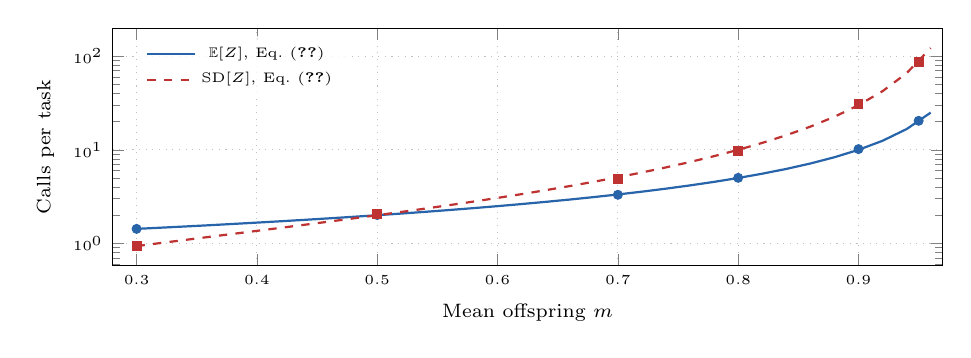
\begin{tikzpicture}
\begin{axis}[xlabel={Mean offspring $m$},ylabel={Calls per task},ymode=log,legend pos=north west,xmin=0.28,xmax=0.97]
\addplot[cblueD,thick] coordinates {(0.3,1.429) (0.32,1.471) (0.34,1.515) (0.36,1.562) (0.38,1.613) (0.4,1.667) (0.42,1.724) (0.44,1.786) (0.46,1.852) (0.48,1.923) (0.5,2) (0.52,2.083) (0.54,2.174) (0.56,2.273) (0.58,2.381) (0.6,2.5) (0.62,2.632) (0.64,2.778) (0.66,2.941) (0.68,3.125) (0.7,3.333) (0.72,3.571) (0.74,3.846) (0.76,4.167) (0.78,4.545) (0.8,5) (0.82,5.556) (0.84,6.25) (0.86,7.143) (0.88,8.333) (0.9,10) (0.92,12.5) (0.94,16.67) (0.96,25)};\addlegendentry{$\E[Z]$, Eq.~(\ref{eq:meanZ})}
\addplot[cblueD,only marks,mark=*,mark size=1.6pt,forget plot] coordinates {(0.3,1.429) (0.5,2.01) (0.7,3.307) (0.8,5.017) (0.9,10.18) (0.95,20.43)};
\addplot[credD,thick,dashed] coordinates {(0.3,0.9352) (0.32,1.009) (0.34,1.087) (0.36,1.172) (0.38,1.263) (0.4,1.361) (0.42,1.467) (0.44,1.583) (0.46,1.709) (0.48,1.848) (0.5,2) (0.52,2.168) (0.54,2.355) (0.56,2.564) (0.58,2.798) (0.6,3.062) (0.62,3.361) (0.64,3.704) (0.66,4.098) (0.68,4.555) (0.7,5.092) (0.72,5.727) (0.74,6.489) (0.76,7.415) (0.78,8.559) (0.8,10) (0.82,11.86) (0.84,14.32) (0.86,17.7) (0.88,22.57) (0.9,30) (0.92,42.39) (0.94,65.97) (0.96,122.5)};\addlegendentry{$\mathrm{SD}[Z]$, Eq.~(\ref{eq:varZ})}
\addplot[credD,only marks,mark=square*,mark size=1.6pt,forget plot] coordinates {(0.3,0.9472) (0.5,2.054) (0.7,4.873) (0.8,9.814) (0.9,30.68) (0.95,87.8)};
\end{axis}
\end{tikzpicture}
\caption{Expected total calls and its standard deviation versus mean offspring for Poisson spawning; lines are theory and markers are simulation.}
\label{fig:branching}
\end{figure}
Criticality is hard to estimate from data near the boundary. Eq.~(\ref{eq:est}) predicts a relative standard error of 0.20 on $\E[Z]$ for $m=0.8$ and $n=500$ offspring observations (95\% half-width 0.39), and simulation gave a mean absolute relative error of 0.18 at $m=0.8$ but 0.63 at $m=0.9$, where 1\% of replications even produced $\hat m\ge1$. A sample of 500 offspring counts therefore pins down $m$ only to about $\pm0.08$ and says little about $\E[Z]$ when $m$ is near 0.9, which is a concrete argument for reporting $m$ with an interval rather than a point estimate.

\subsection{Retries and Cost per Successful Task}
Fig.~\ref{fig:retry} shows that Eq.~(\ref{eq:nu}) matches the simulated task success probability across $R\in\{0,\dots,3\}$ and $p\in[0.05,0.3]$, with a maximum absolute error of 0.18 percentage points over 200{,}000 simulated tasks per point. A single retry lifts $P_s$ at $p=0.2$ from 0.44 to 0.83, and a second to 0.96. Table~\ref{tab:cost} confirms Eq.~(\ref{eq:cost}): simulated cost per success equals $\bar n/(1-p)$ for every $R$ to within 0.6\%, so the benefit of retries is purely reliability.
\begin{figure}[t]
\centering
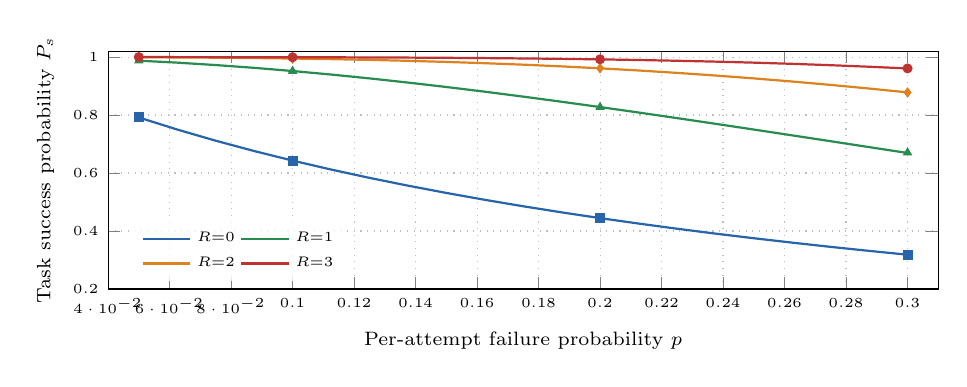
\begin{tikzpicture}
\begin{axis}[xlabel={Per-attempt failure probability $p$},ylabel={Task success probability $P_s$},legend pos=south west,legend columns=2,xmin=0.04,xmax=0.31,ymin=0.2,ymax=1.02]
\addplot[cblueD,thick] coordinates {(0.05,0.7917) (0.0625,0.75) (0.075,0.7115) (0.0875,0.6759) (0.1,0.6429) (0.1125,0.6121) (0.125,0.5833) (0.1375,0.5565) (0.15,0.5313) (0.1625,0.5076) (0.175,0.4853) (0.1875,0.4643) (0.2,0.4444) (0.2125,0.4257) (0.225,0.4079) (0.2375,0.391) (0.25,0.375) (0.2625,0.3598) (0.275,0.3452) (0.2875,0.3314) (0.3,0.3182)};
\addlegendentry{$R{=}0$}
\addplot[cblueD,only marks,mark=square*,mark size=1.6pt,forget plot] coordinates {(0.05,0.792) (0.1,0.6411) (0.2,0.4433) (0.3,0.3182)};
\addplot[cgreenD,thick] coordinates {(0.05,0.9876) (0.0625,0.9808) (0.075,0.9725) (0.0875,0.9629) (0.1,0.9519) (0.1125,0.9398) (0.125,0.9265) (0.1375,0.9121) (0.15,0.8968) (0.1625,0.8806) (0.175,0.8636) (0.1875,0.8459) (0.2,0.8276) (0.2125,0.8088) (0.225,0.7895) (0.2375,0.7699) (0.25,0.75) (0.2625,0.7299) (0.275,0.7097) (0.2875,0.6894) (0.3,0.6691)};
\addlegendentry{$R{=}1$}
\addplot[cgreenD,only marks,mark=triangle*,mark size=1.6pt,forget plot] coordinates {(0.05,0.9877) (0.1,0.952) (0.2,0.8272) (0.3,0.6702)};
\addplot[corangeD,thick] coordinates {(0.05,0.9994) (0.0625,0.9988) (0.075,0.9979) (0.0875,0.9967) (0.1,0.995) (0.1125,0.9929) (0.125,0.9903) (0.1375,0.9871) (0.15,0.9833) (0.1625,0.9789) (0.175,0.9738) (0.1875,0.9679) (0.2,0.9612) (0.2125,0.9538) (0.225,0.9455) (0.2375,0.9364) (0.25,0.9265) (0.2625,0.9157) (0.275,0.904) (0.2875,0.8915) (0.3,0.8782)};
\addlegendentry{$R{=}2$}
\addplot[corangeD,only marks,mark=diamond*,mark size=1.6pt,forget plot] coordinates {(0.05,0.9994) (0.1,0.9947) (0.2,0.9615) (0.3,0.8779)};
\addplot[credD,thick] coordinates {(0.05,1) (0.0625,0.9999) (0.075,0.9998) (0.0875,0.9997) (0.1,0.9995) (0.1125,0.9992) (0.125,0.9988) (0.1375,0.9982) (0.15,0.9975) (0.1625,0.9965) (0.175,0.9953) (0.1875,0.9939) (0.2,0.9921) (0.2125,0.9899) (0.225,0.9873) (0.2375,0.9843) (0.25,0.9808) (0.2625,0.9767) (0.275,0.972) (0.2875,0.9667) (0.3,0.9608)};
\addlegendentry{$R{=}3$}
\addplot[credD,only marks,mark=*,mark size=1.6pt,forget plot] coordinates {(0.05,1) (0.1,0.9995) (0.2,0.9923) (0.3,0.9609)};

\end{axis}
\end{tikzpicture}
\caption{Task success probability versus failure probability for retry budgets $R=0,\dots,3$ ($\bar n=5$); lines are Eq.~(\ref{eq:nu}) and markers are simulation.}
\label{fig:retry}
\end{figure}
\begin{table}[t]
\caption{Calls per successful task ($\bar n=5$): Eq.~(\ref{eq:cost}) versus simulation}
\label{tab:cost}
\centering
\footnotesize
\begin{tabular}{rrrrrr}
\toprule
 & Eq. & \multicolumn{4}{c}{Simulation} \\
\cmidrule(lr){3-6}
$p$ & $\bar n/(1-p)$ & $R{=}0$ & $R{=}1$ & $R{=}2$ & $R{=}3$ \\
\midrule
0.05 & 5.263 & 5.264 & 5.274 & 5.247 & 5.270 \\
0.10 & 5.556 & 5.586 & 5.547 & 5.561 & 5.568 \\
0.20 & 6.250 & 6.257 & 6.265 & 6.255 & 6.254 \\
0.30 & 7.143 & 7.141 & 7.128 & 7.131 & 7.140 \\
\bottomrule
\end{tabular}
\end{table}

\subsection{Fork-Join Effects}
Fig.~\ref{fig:forkjoin} varies the fixed fan-out $K$ at constant arrival rate $\lambda=0.28$ tasks/s ($\rho_L=0.55$, tool pool of 128 servers so that $\rho_T\le0.37$). Mean latency rises from 21.3\,s at $K=1$ to 48.3\,s at $K=32$ and p99 from 95\,s to 210\,s, with the increment per doubling of $K$ growing from 2.9\,s to 8.3\,s, a consequence of lognormal service times whose maximum grows faster than logarithmically. The full model tracks the simulator within 0.4\% on the mean and 1.0\% on p99 at every $K$, whereas an otherwise identical model without the join (a single tool call per step) is flat in $K$ and underestimates the mean by 56\% at $K=32$. Fan-out is thus a first-order tail-latency parameter even when the tool pool is lightly loaded.
\begin{figure}[t]
\centering
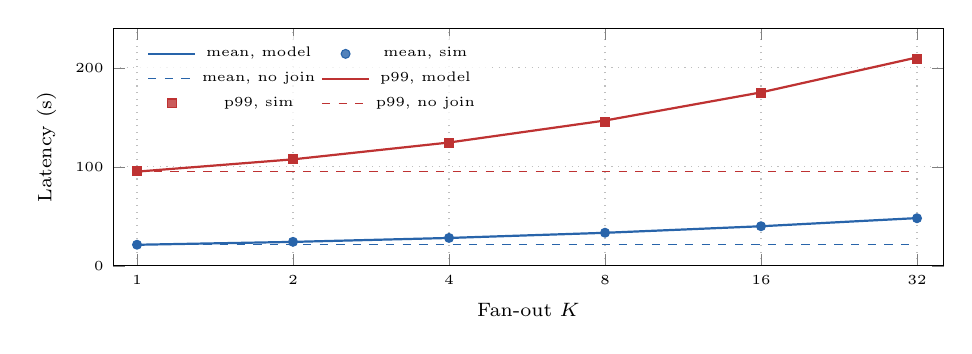
\begin{tikzpicture}
\begin{axis}[xlabel={Fan-out $K$},ylabel={Latency (s)},xmode=log,log basis x=2,xtick={1,2,4,8,16,32},xticklabels={1,2,4,8,16,32},legend pos=north west,legend columns=2,ymin=0,ymax=240,xmin=0.9,xmax=36]
\addplot[cblueD,thick] coordinates {(1,21.33) (2,24.24) (4,28.22) (8,33.42) (16,40.04) (32,48.28)};\addlegendentry{mean, model}
\addplot[cblueD,only marks,mark=*,mark size=1.6pt] coordinates {(1,21.39) (2,24.31) (4,28.26) (8,33.5) (16,40.06) (32,48.12)};\addlegendentry{mean, sim}
\addplot[cblueD,dashed] coordinates {(1,21.33) (2,21.33) (4,21.33) (8,21.33) (16,21.33) (32,21.33)};\addlegendentry{mean, no join}
\addplot[credD,thick] coordinates {(1,95.2) (2,107.6) (4,124.6) (8,146.8) (16,175.2) (32,210.5)};\addlegendentry{p99, model}
\addplot[credD,only marks,mark=square*,mark size=1.6pt] coordinates {(1,95.77) (2,108.2) (4,124.1) (8,145.7) (16,174.5) (32,208.5)};\addlegendentry{p99, sim}
\addplot[credD,dashed] coordinates {(1,95.2) (2,95.2) (4,95.2) (8,95.2) (16,95.2) (32,95.2)};\addlegendentry{p99, no join}
\end{axis}
\end{tikzpicture}
\caption{Mean and p99 latency of successful tasks versus fan-out at fixed arrival rate. Dashed curves omit the join and are flat in $K$.}
\label{fig:forkjoin}
\end{figure}

\subsection{End-to-End Validation}
Table~\ref{tab:valid} and Fig.~\ref{fig:load} compare predicted and simulated latency as load increases. For $\rho_L\le0.8$ the largest errors over all three profiles are 2.3\% (mean), 4.6\% (p95), and 9.6\% (p99), and nearly all are underestimates; at $\rho_L\le0.5$ every error is at most 0.5\%. Predicted success probability matched simulation to within 0.1 percentage points in every configuration (for example 0.951, 0.975, and 0.969 for P1, P2, and P3). At $\rho_L=0.9$ the model underestimates the mean by 0.9--8.7\%, p95 by 4.8--17.3\%, and p99 by 10.8--32.2\%, while the seed-to-seed standard deviation of simulated p99 reaches 102\,s for P1, so part of the gap is sampling noise but the sign is consistent. The likely cause is that the exponential-tail waiting approximation of Eq.~(\ref{eq:wait}) is too light for lognormal service times near saturation and that queue correlation across successive calls of the same task is ignored.
\begin{table*}[t]
\caption{Model versus simulation across load (errors are model minus simulation, in percent; $\rho_L$ and $\rho_T$ are pool utilizations)}
\label{tab:valid}
\centering
\footnotesize
\begin{tabular}{llrrrrrrr}
\toprule
Profile & $\rho_L$ & $\rho_T$ & Mean sim (s) & Err (\%) & p95 sim (s) & Err (\%) & p99 sim (s) & Err (\%) \\
\midrule
P1 & 0.5 & 0.08 & 31.9 & $-$0.4 & 93.9 & $-$0.2 & 143.7 & +0.1 \\
 & 0.7 & 0.12 & 34.2 & $-$0.8 & 101.9 & $-$1.9 & 157.0 & $-$2.4 \\
 & 0.8 & 0.13 & 38.7 & $-$2.3 & 116.5 & $-$4.6 & 188.4 & $-$9.6 \\
 & 0.9 & 0.15 & 55.9 & $-$8.7 & 181.0 & $-$17.3 & 338.4 & $-$32.2 \\
\midrule
P2 & 0.5 & 0.25 & 25.0 & $-$0.2 & 71.1 & $-$0.1 & 108.5 & $-$0.1 \\
 & 0.7 & 0.35 & 25.9 & +0.3 & 74.2 & $-$0.2 & 114.2 & $-$1.0 \\
 & 0.8 & 0.40 & 28.2 & $-$0.7 & 81.1 & $-$1.9 & 125.5 & $-$3.4 \\
 & 0.9 & 0.45 & 35.1 & $-$0.9 & 103.6 & $-$4.8 & 168.3 & $-$10.8 \\
\midrule
P3 & 0.5 & 0.17 & 23.3 & $-$0.2 & 67.7 & $-$0.1 & 104.2 & $-$0.5 \\
 & 0.7 & 0.23 & 24.9 & $-$0.8 & 72.6 & $-$1.4 & 114.2 & $-$4.2 \\
 & 0.8 & 0.27 & 27.6 & $-$1.6 & 81.4 & $-$3.6 & 130.1 & $-$7.8 \\
 & 0.9 & 0.30 & 37.7 & $-$5.7 & 116.1 & $-$11.6 & 198.8 & $-$21.1 \\
\bottomrule
\end{tabular}
\end{table*}
\begin{figure}[t]
\centering
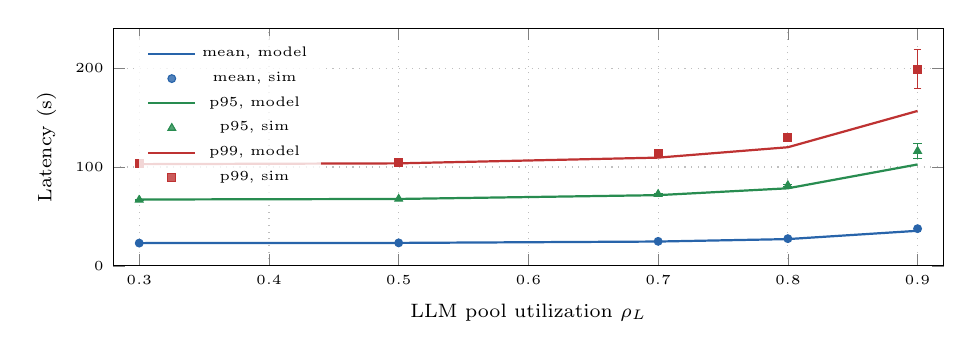
\begin{tikzpicture}
\begin{axis}[xlabel={LLM pool utilization $\rho_L$},ylabel={Latency (s)},legend pos=north west,xmin=0.28,xmax=0.92,ymin=0]
\addplot[cblueD,thick] coordinates {(0.3,23.05) (0.5,23.25) (0.7,24.64) (0.8,27.11) (0.9,35.51)};\addlegendentry{mean, model}
\addplot[cblueD,only marks,mark=*,mark size=1.4pt,error bars/.cd,y dir=both,y explicit] coordinates {(0.3,23.07) +- (0,0.0726) (0.5,23.29) +- (0,0.108) (0.7,24.85) +- (0,0.361) (0.8,27.56) +- (0,0.424) (0.9,37.66) +- (0,2.15)};\addlegendentry{mean, sim}
\addplot[cgreenD,thick] coordinates {(0.3,67.14) (0.5,67.7) (0.7,71.56) (0.8,78.48) (0.9,102.6)};\addlegendentry{p95, model}
\addplot[cgreenD,only marks,mark=triangle*,mark size=1.6pt,error bars/.cd,y dir=both,y explicit] coordinates {(0.3,66.8) +- (0,0.341) (0.5,67.74) +- (0,0.516) (0.7,72.56) +- (0,0.716) (0.8,81.39) +- (0,0.877) (0.9,116.1) +- (0,7.48)};\addlegendentry{p95, sim}
\addplot[credD,thick] coordinates {(0.3,102.9) (0.5,103.7) (0.7,109.5) (0.8,120) (0.9,156.7)};\addlegendentry{p99, model}
\addplot[credD,only marks,mark=square*,mark size=1.4pt,error bars/.cd,y dir=both,y explicit] coordinates {(0.3,103.2) +- (0,0.941) (0.5,104.2) +- (0,0.72) (0.7,114.2) +- (0,2.77) (0.8,130.1) +- (0,2.1) (0.9,198.8) +- (0,19.7)};\addlegendentry{p99, sim}
\end{axis}
\end{tikzpicture}
\caption{Latency of successful tasks versus LLM utilization for profile P3 (error bars: one standard deviation over 4 seeds).}
\label{fig:load}
\end{figure}

\subsection{Bottleneck Analysis}
Table~\ref{tab:bott} applies Eq.~(\ref{eq:lamstar}) to each profile. The LLM pool saturates first for P1, P2, and P3 because tool calls are shorter and the tool pools are larger. Shrinking the P2 tool pool to $k_T=8$ moves the bottleneck to the tools: $\lambda^\ast_T=0.315$ is half of $\lambda^\ast_L=0.629$, and the model error at $0.9\lambda^\ast$ grows to $-21.6\%$ on the mean and $-39.6\%$ on p99, compared with $-0.9\%$ and $-10.8\%$ when the LLM is the bottleneck at the same relative load. The independence assumption between the $K{=}6$ parallel calls is weakest when they queue in the same congested pool, which identifies fork-join on a saturated pool as the least accurate regime of the model. We conjecture that the cause is batch release: the siblings of a fork arrive at the pool together, so later siblings queue behind earlier ones, whereas Eq.~(\ref{eq:wait}) assumes Poisson arrivals at the pool. This would explain why the error is an underestimate even though independent-maximum approximations are conservative when tasks go to distinct servers \cite{thomasian2014forkjoin}.
\begin{table}[t]
\caption{Saturation analysis at $0.9\lambda^\ast$ (errors: model minus simulation, \%)}
\label{tab:bott}
\centering
\footnotesize
\setlength{\tabcolsep}{2.5pt}
\begin{tabular}{lrrrrlrrr}
\toprule
Profile & $c_L$ & $c_T$ & $\lambda^\ast_L$ & $\lambda^\ast_T$ & Bott. & $\rho_L^{\mathrm{sim}}$ & Mean & p99 \\
\midrule
P1 & 8.27 & 8.3 & 0.322 & 1.935 & LLM & 0.90 & $-$8.7 & $-$32.2 \\
P2 & 4.24 & 25.4 & 0.629 & 1.258 & LLM & 0.90 & $-$0.9 & $-$10.8 \\
P2 ($k_T{=}8$) & 4.24 & 25.4 & 0.629 & 0.315 & Tool & 0.45 & $-$21.6 & $-$39.6 \\
P3 & 5.27 & 10.5 & 0.506 & 1.519 & LLM & 0.91 & $-$5.7 & $-$21.1 \\
\bottomrule
\end{tabular}
\end{table}

\subsection{Depth, Runtime, and Scalability}
At fixed $\lambda=0.1$ tasks/s on P3, increasing the mean workflow length from $\bar n=2$ to $16$ raises predicted mean latency from 9.4\,s to 69.4\,s and p99 from 40\,s to 302\,s, lowers $P_s$ from 0.987 to 0.907, and raises calls per success from 2.2 to 17.4 in line with Eq.~(\ref{eq:cost}); $\rho_L$ grows from 0.08 to 0.59, so depth also consumes capacity. Evaluating the model for one configuration takes 0.52\,s (0.29\,s for the $K=32$ configuration) on a single core, independent of $\lambda$ and of the number of simulated tasks, versus 2.2\,s for one 30{,}000-task simulation. The speedup is modest here because the simulator is small, but the model returns a smooth distribution without sampling noise, which matters at p99.

\subsection{Sub-Agent Trees}
Table~\ref{tab:tree} and Fig.~\ref{fig:treeplot} compare the recursive model of Section~\ref{sec:tree} with a simulator that implements delegation, joins, and failure propagation. Agents per tree (Eq.~(\ref{eq:agents})) agree with simulation to within 0.5\% in all nine configurations, for example 1.42 against 1.42 at $m=0.3$ and 1.96 against 1.96 at $m=0.5$, and tree success probability (Eq.~(\ref{eq:treesucc})) agrees to within 0.1 percentage points. Latency errors follow the pattern seen for single chains but are larger at high load: at $\rho_L\le0.5$ all errors are at most 1.0\%, at $\rho_L=0.7$ the mean, p95, and p99 errors are at most 3.5\%, 4.2\%, and 6.2\%, and at $\rho_L=0.8$ they reach 6.5\%, 9.3\%, and 14.1\% for $m=0.5$. All errors are underestimates except for sampling noise at light load. Delegation matters even at modest $m$: raising $m$ from 0 to 0.5 at $\rho_L=0.5$ multiplies mean latency from 14.1\,s to 25.0\,s and p99 from 61.4\,s to 117.9\,s, a 1.8-fold and 1.9-fold increase, while consuming 1.96 times as many agent chains. The growth in tail error with $m$ is consistent with the ignored correlation of simultaneous sub-agent starts, which produces short bursts at the pools.
\begin{figure}[t]
\centering
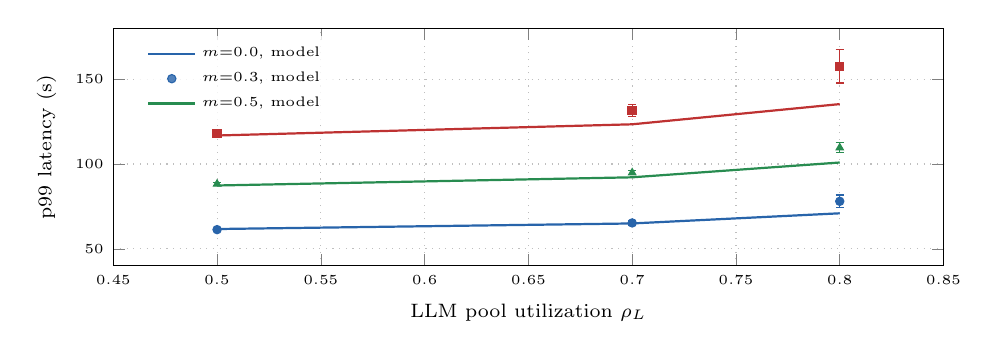
\begin{tikzpicture}
\begin{axis}[xlabel={LLM pool utilization $\rho_L$},ylabel={p99 latency (s)},legend pos=north west,legend columns=1,xmin=0.45,xmax=0.85,ymin=40]
\addplot[cblueD,thick] coordinates {(0.5,61.72) (0.7,65) (0.8,70.98)};\addlegendentry{$m{=}0.0$, model}
\addplot[cblueD,only marks,mark=*,mark size=1.5pt,error bars/.cd,y dir=both,y explicit] coordinates {(0.5,61.37) +- (0,0.786) (0.7,65.31) +- (0,1.48) (0.8,78.04) +- (0,3.73)};
\addplot[cgreenD,thick] coordinates {(0.5,87.36) (0.7,92.18) (0.8,100.9)};\addlegendentry{$m{=}0.3$, model}
\addplot[cgreenD,only marks,mark=triangle*,mark size=1.5pt,error bars/.cd,y dir=both,y explicit] coordinates {(0.5,88.24) +- (0,1.08) (0.7,94.91) +- (0,1.22) (0.8,109.6) +- (0,2.94)};
\addplot[credD,thick] coordinates {(0.5,116.8) (0.7,123.4) (0.8,135.3)};\addlegendentry{$m{=}0.5$, model}
\addplot[credD,only marks,mark=square*,mark size=1.5pt,error bars/.cd,y dir=both,y explicit] coordinates {(0.5,117.9) +- (0,1.79) (0.7,131.6) +- (0,3.67) (0.8,157.5) +- (0,9.76)};
\end{axis}
\end{tikzpicture}
\caption{p99 latency of successful sub-agent trees versus LLM utilization for mean delegation $m=0,0.3,0.5$; lines are the model and markers are simulation with 95\% confidence intervals.}
\label{fig:treeplot}
\end{figure}

\subsection{Service-Time Variability}
The ablation of Section~\ref{sec:compare} showed little sensitivity to replacing lognormal with exponential service, but the LLM coefficient of variation there was already 0.9. Table~\ref{tab:cv} varies it from 0.5 to 2.5 at fixed means. The model underestimates for low variability ($-5.4\%$ mean and $-9.7\%$ p99 at CV 0.5), is closest around CV 1.5 ($+7.7\%$ mean, $-0.3\%$ p99), and overestimates for heavy tails: at CV 2.5 the mean is overestimated by 31.0\%, p95 by 24.6\%, and p99 by 14.2\%. The Allen--Cunneen factor $(c_a^2+c_s^2)/2$ grows linearly in $c_s^2$, but in the simulator a heavy-tailed service distribution has most of its mass on short jobs, so the effective queueing delay grows more slowly. Practitioners should therefore expect conservative predictions for heavy-tailed LLM service times and optimistic predictions for near-deterministic ones. The sign change in the error implies that a single margin $\delta$ in Eq.~(\ref{eq:slo}) is not universally safe, which is the main reason to calibrate $\delta$ per workload.

\subsection{Bursty Arrivals}
Table~\ref{tab:bracket} evaluates the bracketing hypothesis of Eq.~(\ref{eq:bracket}) for burst factors 4 and 8, three load levels, and two modulation speeds (mean high-state sojourn of 50\,s and 200\,s, with low-state sojourn three times longer). In all 12 settings the simulated mean and p99 lie between the Poisson prediction and the quasi-static prediction, where the latter is defined. In the two settings where the high-state rate exceeds capacity ($\rho_L=0.4$, $\beta=8$, so $\rho_L(r_1)=1.16$) the quasi-static predictor is undefined, and the simulated p99 is 146\,s for fast and 326\,s for slow modulation, against 103\,s for the Poisson predictor; the slow case shows that queues grow throughout a burst, as expected. Slower modulation moves the simulation toward the quasi-static prediction: at $\rho_L=0.3$ and $\beta=8$ the simulated mean is 24.7\,s (fast) and 27.4\,s (slow) between 23.1\,s (Poisson) and 29.4\,s (quasi-static). The bracket is tight at low load (width below 1\,s for $\rho_L=0.2$) and wide when the high state approaches saturation (for example 23.1\,s to 31.8\,s at $\rho_L=0.4$, $\beta=4$), so it is useful as a screening tool: if the bracket is narrow the Poisson model suffices, and if the quasi-static predictor is undefined the system needs burst-aware provisioning. Twelve settings from one profile do not establish the bracket as a general property, and we state it as an empirical regularity.

\subsection{Capacity Planning}
Table~\ref{tab:slo} uses Eq.~(\ref{eq:slo}) to find the maximum arrival rate meeting a p99 target of 150\,s for four LLM pool sizes. Trusting the model ($\delta=1$) selects utilizations of 0.86--0.92 and the simulated p99 then exceeds the target in all four cases, by 18\% to 26\% (176--189\,s against 150\,s), consistent with the underestimation near saturation seen in Table~\ref{tab:valid}. With $\delta=0.85$ the simulated p99 was 142\,s, 142\,s, 142\,s, and 139\,s for $k_L=6,8,10,12$, below the target on average, although the 95\% interval for $k_L=10$ (142\,s $\pm$ 8\,s) touches it. The $\rho_L=0.7$ rule is safe (p99 of 107--119\,s) but conservative, and the margin rule admits 13\% to 26\% more load, a gain that grows with pool size because the queueing penalty at a given utilization shrinks as $k_L$ grows. The margin of 0.85 was chosen from the errors of Section~\ref{sec:results} on the same profile family, so this experiment shows that a validation-derived margin transfers to other pool sizes, not that it transfers to other workloads.

\begin{table*}[t]
\caption{Sub-agent tree validation ($\bar n=3$, $\mu_K=2$): agents per tree $M$, tree success probability $S$, and latency of successful trees. Simulation entries are means $\pm$ 95\% confidence half-widths over 8 seeds; errors are model minus simulation, in percent}
\label{tab:tree}
\centering
\footnotesize
\setlength{\tabcolsep}{3.2pt}
\begin{tabular}{rrrrrrrrrrrr}
\toprule
 & & \multicolumn{2}{c}{$M$} & \multicolumn{2}{c}{$S$} & \multicolumn{2}{c}{Mean (s)} & \multicolumn{2}{c}{p95 (s)} & \multicolumn{2}{c}{p99 (s)} \\
\cmidrule(lr){3-4}\cmidrule(lr){5-6}\cmidrule(lr){7-8}\cmidrule(lr){9-10}\cmidrule(lr){11-12}
$m$ & $\rho_L$ & Eq. & Sim & Eq. & Sim & Sim & Err & Sim & Err & Sim & Err \\
\midrule
0.0 & 0.5 & 1.00 & 1.00 & 0.981 & 0.981 & 14.1$\pm$0.1 & +0.3 & 40.0$\pm$0.3 & +0.6 & 61.4$\pm$0.8 & +0.6 \\
0.0 & 0.7 & 1.00 & 1.00 & 0.981 & 0.982 & 14.9$\pm$0.2 & +0.3 & 42.5$\pm$0.6 & +0.1 & 65.3$\pm$1.5 & $-$0.5 \\
0.0 & 0.8 & 1.00 & 1.00 & 0.981 & 0.981 & 16.9$\pm$0.4 & $-$2.6 & 48.8$\pm$1.7 & $-$4.7 & 78.0$\pm$3.7 & $-$9.0 \\
\midrule
0.3 & 0.5 & 1.42 & 1.42 & 0.973 & 0.973 & 19.6$\pm$0.1 & $-$0.9 & 57.3$\pm$0.8 & $-$1.0 & 88.2$\pm$1.1 & $-$1.0 \\
0.3 & 0.7 & 1.42 & 1.42 & 0.973 & 0.973 & 20.9$\pm$0.2 & $-$1.5 & 61.0$\pm$0.6 & $-$1.8 & 94.9$\pm$1.2 & $-$2.9 \\
0.3 & 0.8 & 1.42 & 1.42 & 0.973 & 0.973 & 23.1$\pm$0.3 & $-$2.1 & 68.6$\pm$1.4 & $-$4.3 & 109.6$\pm$2.9 & $-$7.9 \\
\midrule
0.5 & 0.5 & 1.96 & 1.97 & 0.963 & 0.964 & 25.0$\pm$0.1 & $-$1.0 & 75.6$\pm$0.4 & $-$1.3 & 117.9$\pm$1.8 & $-$0.9 \\
0.5 & 0.7 & 1.96 & 1.96 & 0.963 & 0.963 & 27.1$\pm$0.4 & $-$3.5 & 82.4$\pm$1.8 & $-$4.2 & 131.6$\pm$3.7 & $-$6.2 \\
0.5 & 0.8 & 1.96 & 1.96 & 0.963 & 0.962 & 30.8$\pm$1.2 & $-$6.5 & 95.5$\pm$4.5 & $-$9.3 & 157.5$\pm$9.8 & $-$14.1 \\
\bottomrule
\end{tabular}
\end{table*}
\begin{table*}[t]
\caption{Sensitivity to LLM service-time variability (P3, $\rho_L=0.8$, 8 seeds, simulation entries are means $\pm$ 95\% confidence half-widths; errors are model minus simulation, in percent)}
\label{tab:cv}
\centering
\footnotesize
\begin{tabular}{rrrrrrrrrr}
\toprule
 & \multicolumn{3}{c}{Mean (s)} & \multicolumn{3}{c}{p95 (s)} & \multicolumn{3}{c}{p99 (s)} \\
\cmidrule(lr){2-4}\cmidrule(lr){5-7}\cmidrule(lr){8-10}
CV$_L$ & Sim & Model & Err & Sim & Model & Err & Sim & Model & Err \\
\midrule
0.5 & 27.3$\pm$0.5 & 25.9 & $-$5.4 & 79.3$\pm$1.7 & 73.8 & $-$7.0 & 124.6$\pm$4.5 & 112.5 & $-$9.7 \\
0.9 & 27.6$\pm$0.4 & 27.1 & $-$1.8 & 81.7$\pm$1.0 & 78.5 & $-$3.9 & 130.3$\pm$2.3 & 120.0 & $-$7.9 \\
1.5 & 28.2$\pm$0.6 & 30.3 & +7.7 & 86.0$\pm$2.3 & 90.3 & +4.9 & 140.1$\pm$5.7 & 139.7 & $-$0.3 \\
2.5 & 30.0$\pm$0.9 & 39.3 & +31.0 & 97.0$\pm$3.3 & 120.8 & +24.6 & 167.7$\pm$11.6 & 191.5 & +14.2 \\
\bottomrule
\end{tabular}
\end{table*}
\begin{table*}[t]
\caption{Bracketing of latency under MMPP arrivals (P3). $\sigma$ is the state-switching rate out of the high state (mean high-state sojourn $1/\sigma$); Poisson and quasi-static (QS) predictors are Eqs.~(\ref{eq:qs}) and the Poisson predictor of Section~\ref{sec:burst}; QS is undefined (--) when the high-state rate saturates the LLM pool; simulation entries are means $\pm$ 95\% confidence half-widths over 6 seeds}
\label{tab:bracket}
\centering
\footnotesize
\begin{tabular}{rrrrrrrrrr}
\toprule
 & & & \multicolumn{3}{c}{Mean latency (s)} & \multicolumn{3}{c}{p99 latency (s)} \\
\cmidrule(lr){4-6}\cmidrule(lr){7-9}
$\sigma$ (1/s) & $\rho_L$ & $\beta$ & Poisson & Sim & QS & Poisson & Sim & QS \\
\midrule
0.02 & 0.2 & 4 & 23.0 & 23.0$\pm$0.1 & 23.1 & 103 & 103$\pm$2 & 103 \\
0.02 & 0.2 & 8 & 23.0 & 23.2$\pm$0.1 & 23.4 & 103 & 103$\pm$1 & 104 \\
0.02 & 0.3 & 4 & 23.1 & 23.2$\pm$0.2 & 23.8 & 103 & 104$\pm$2 & 106 \\
0.02 & 0.3 & 8 & 23.1 & 24.7$\pm$0.3 & 29.4 & 103 & 112$\pm$1 & 133 \\
0.02 & 0.4 & 4 & 23.1 & 24.7$\pm$0.3 & 31.8 & 103 & 112$\pm$4 & 151 \\
0.02 & 0.4 & 8 & 23.1 & 30.2$\pm$0.4 & -- & 103 & 146$\pm$6 & -- \\
\midrule
0.005 & 0.2 & 4 & 23.0 & 23.0$\pm$0.1 & 23.1 & 103 & 103$\pm$1 & 103 \\
0.005 & 0.2 & 8 & 23.0 & 23.4$\pm$0.1 & 23.4 & 103 & 104$\pm$2 & 104 \\
0.005 & 0.3 & 4 & 23.1 & 23.7$\pm$0.1 & 23.8 & 103 & 106$\pm$1 & 106 \\
0.005 & 0.3 & 8 & 23.1 & 27.4$\pm$0.4 & 29.4 & 103 & 131$\pm$5 & 133 \\
0.005 & 0.4 & 4 & 23.1 & 27.9$\pm$1.1 & 31.8 & 103 & 137$\pm$11 & 151 \\
0.005 & 0.4 & 8 & 23.1 & 51.1$\pm$1.2 & -- & 103 & 326$\pm$13 & -- \\
\bottomrule
\end{tabular}
\end{table*}
\begin{table}[t]
\caption{Capacity planning for a p99 target of 150\,s (P3, $k_T=2k_L$). Arrival rates $\lambda$ are in tasks/s. Naive: $\rho_L=0.7$ rule. Model: Eq.~(\ref{eq:slo}) with $\delta=1$. Margin: $\delta=0.85$. Simulated p99 (s) is the mean $\pm$ 95\% confidence half-width over 8 seeds; the last column is the throughput gain of the margin rule over the naive rule (\%)}
\label{tab:slo}
\centering
\footnotesize
\setlength{\tabcolsep}{2.5pt}
\begin{tabular}{rrrrrrrr}
\toprule
 & \multicolumn{3}{c}{$\lambda$ (tasks/s)} & \multicolumn{3}{c}{Simulated p99 (s)} & \\
\cmidrule(lr){2-4}\cmidrule(lr){5-7}
$k_L$ & Naive & Model & Margin & Naive & Model & Margin & Gain \\
\midrule
6 & 0.266 & 0.327 & 0.301 & 119$\pm$2 & 180$\pm$12 & 142$\pm$4 & +13.3 \\
8 & 0.355 & 0.451 & 0.423 & 113$\pm$2 & 189$\pm$18 & 142$\pm$4 & +19.4 \\
10 & 0.443 & 0.576 & 0.546 & 107$\pm$2 & 176$\pm$9 & 142$\pm$8 & +23.2 \\
12 & 0.532 & 0.701 & 0.670 & 107$\pm$2 & 178$\pm$22 & 139$\pm$5 & +25.9 \\
\bottomrule
\end{tabular}
\end{table}

\section{Comparative Analysis}\label{sec:compare}
Table~\ref{tab:ablation} removes one component of the model at a time for P3 at $\rho_L=0.8$, where the simulated reference is 27.6\,s mean, 81.4\,s p95, and 130.1\,s p99. The full model has errors of $-1.6\%$, $-3.6\%$, and $-7.8\%$. Dropping queueing (service times only) is the most damaging change ($-16.4\%$ mean, $-21.0\%$ p99), followed by dropping retries ($-10.6\%$, $-16.1\%$) and dropping the join ($-9.3\%$, $-14.8\%$). A mean-value model, which sums mean waits and service times as a Little's-law style capacity calculation would, errs by $-8.8\%$ on the mean and cannot produce percentiles at all. Replacing the lognormal service times with exponential ones changes errors by under one point, because the LLM coefficient of variation (0.9) is already close to 1; this ablation says nothing about heavier tails, which were not tested. In short, each structural component contributes a systematic error of 9--21\% if omitted, and none of the alternatives matches the full model in the tail.
\begin{table}[t]
\caption{Ablation and baseline comparison, P3 at $\rho_L=0.8$ (errors: model minus simulation, \%)}
\label{tab:ablation}
\centering
\scriptsize
\setlength{\tabcolsep}{1.8pt}
\begin{tabular}{lrrrrrr}
\toprule
Variant & Mean & Err & p95 & Err & p99 & Err \\
\midrule
Simulation & 27.6 & -- & 81.4 & -- & 130.1 & -- \\
\midrule
Full model & 27.1 & $-$1.6 & 78.5 & $-$3.6 & 120.0 & $-$7.8 \\
No queueing (service only) & 23.0 & $-$16.4 & 67.1 & $-$17.5 & 102.8 & $-$21.0 \\
No fork-join (single tool) & 25.0 & $-$9.3 & 72.5 & $-$11.0 & 110.9 & $-$14.8 \\
No retries ($R{=}0,p{=}0$) & 24.7 & $-$10.6 & 71.4 & $-$12.3 & 109.2 & $-$16.1 \\
Exponential service (M/M/$k$) & 26.9 & $-$2.4 & 77.9 & $-$4.3 & 119.1 & $-$8.5 \\
Mean-value (no distribution) & 25.1 & $-$8.8 & -- & -- & -- & -- \\
\bottomrule
\end{tabular}
\end{table}

\section{Discussion and Deployment Considerations}\label{sec:discuss}
\textbf{What the model is good for.} The model is most useful for relative questions at moderate load: how much p99 latency a given increase in fan-out, depth, or delegation costs, which pool saturates first, and how many LLM replicas a target requires. For these questions its errors (below 10\% in p99 up to $\rho_L=0.8$ for chains) are smaller than the effects of the design choices being compared (tens of percent to multiples; see Fig.~\ref{fig:forkjoin} and Table~\ref{tab:tree}).

\textbf{Using it in practice.} A deployment workflow follows Fig.~\ref{fig:pipeline}: estimate the structural parameters ($\bar n$, $\mu_K$, $m$, $p$) and service-time moments from production logs; compute $\lambda^\ast$ with Eq.~(\ref{eq:lamstar}) to identify the bottleneck; check burstiness with the bracket of Section~\ref{sec:burst}; and size the pools with Eq.~(\ref{eq:slo}) using a margin calibrated against a simulator or a canary. Because the inputs to Eq.~(\ref{eq:est}) are offspring counts, the confidence interval on $m$ should be reported with every capacity estimate, since Section~\ref{sec:results} shows that $\E[Z]$ is poorly determined by a few hundred tasks when $m\ge0.9$.

\textbf{Relation to measured workloads.} The structural parameters used here are of the same order as those reported for coding agents, where requests average 8.8 LLM calls \cite{zhu2026tracelab}, comparable to $\bar n=8$ in profile P1. Two measured features differ from our assumptions. First, tool latencies in that trace are far heavier-tailed than the lognormal with coefficient of variation 1.5 used here, since calls longer than one minute account for 4\% of calls and 85\% of tool time \cite{zhu2026tracelab}; our sensitivity study (Table~\ref{tab:cv}) varied only the LLM service variability, so the accuracy of the model under such tool tails is untested. Second, non-LLM components dominate latency in half of the applications of a recent benchmark \cite{chang2026agentic}, which suggests that the tool-bound regime, where Table~\ref{tab:bott} shows the model to be least accurate, is common in practice. Both points argue for calibrating and re-validating the model on traces before using it for capacity decisions.

\textbf{Operational levers.} The results suggest three levers in order of effect. Reducing delegation $m$ lowers both load and tail (Table~\ref{tab:tree}); capping fan-out or using hedged tool calls limits fork-join tail growth (Fig.~\ref{fig:forkjoin}); and adding retries improves reliability but leaves cost per success unchanged (Eq.~(\ref{eq:cost})), so retries should be set by reliability targets and not by cost. These are model-derived observations about the simulated system and need confirmation on real deployments.

\textbf{Threats to validity.} Internal validity is limited by the use of 4--8 seeds and by tail estimates at $\rho_L=0.9$, whose confidence intervals are wide (a standard deviation of 102\,s on a p99 of 338\,s for P1). External validity is limited by synthetic parameters, three structural profiles, and one family of service-time distributions; construct validity is limited by comparing the model with a simulator that shares its structural assumptions.

\section{Limitations}\label{sec:limits}
\textbf{Synthetic workloads.} The central limitation is that no real agent traces were collected: distributions, parameters, and structural profiles are assumed. The results quantify approximation error against a simulator that shares the model's independence structure for step counts and failures, so they are an upper bound on agreement with real systems, not evidence of fit. Distribution selection by maximum likelihood and AIC \cite{akaike1974aic,clauset2009power}, and checking for heavy tails beyond lognormal, remain to be done on measured data.

\textbf{Bursty arrivals.} The stationary model fails under bursty arrivals. Arrivals were generated by a two-state MMPP \cite{fischer1993mmpp} with burst factor $\beta$, the ratio of high to low rate. In the conference-version experiment with mean sojourns of 50\,s and 150\,s, at $\rho_L=0.7$ and $\beta=4$ the simulated mean was 58.6\,s against a predicted 24.6\,s and the simulated p99 was 425\,s against 110\,s, and replacing $c_a^2$ in Eq.~(\ref{eq:ac}) by the measured interarrival SCV closed less than 5\% of the gap at $\rho_L=0.8$. Section~\ref{sec:burst} gives a bracketing treatment that is informative only when the high-state load remains below saturation; self-exciting arrival models such as Hawkes processes \cite{hawkes1971spectra,bacry2015hawkes} or time-varying fluid approximations would be needed for an accurate point prediction. Table~\ref{tab:burst} shows the size of the failure of the Poisson predictor.

\textbf{Load-independent retries.} The failure probability $p$ is a constant. In production systems, timeouts and client retries make retries depend on load: in an analysis of public incident reports, retry-driven workload amplification was the most common mechanism sustaining metastable failures, present in more than half of the studied incidents \cite{huang2022metastable}, where a system remains overloaded after the trigger is removed \cite{bronson2021metastable}. Eq.~(\ref{eq:cost}) still gives calls per success for a fixed $p$, but if $p$ increases with utilization, the load equations (\ref{eq:load}) become a fixed point that may have more than one solution; we do not analyze this regime.

\textbf{Literature coverage.} The related-work search used general web search and publisher, Crossref, arXiv, and proceedings records accessed on 23 October 2026, not a systematic database protocol, and forward-citation searches were not performed. Several of the most relevant recent works are preprints whose content may change.

\textbf{Other approximations.} The model ignores correlation among queue states seen by successive calls of one task, assumes independent tool responses within a join, treats service times as independent of retry and failure, covers chains of steps with Poisson tool fan-out and Poisson delegation (sub-agent trees are coupled to the queueing layer only through the mean load factor $M$), and does not model batching effects inside LLM servers \cite{kwon2023vllm,yu2022orca}, where service time depends on load.
\begin{table}[t]
\caption{Effect of bursty (MMPP) arrivals on a Poisson-assuming model, P3; $\beta$ is the burst factor (1 = Poisson)}
\label{tab:burst}
\centering
\footnotesize
\setlength{\tabcolsep}{2pt}
\begin{tabular}{rrrrrrr}
\toprule
 & & & \multicolumn{2}{c}{Mean (s)} & \multicolumn{2}{c}{p99 (s)} \\
\cmidrule(lr){4-5}\cmidrule(lr){6-7}
$\rho_L$ & $\beta$ & SCV & Sim & Model & Sim & Model \\
\midrule
0.5 & 1 & 1.00 & 23.3 & 23.3 & 104 & 104 \\
0.5 & 4 & 1.77 & 29.2 & 23.3 & 144 & 104 \\
0.5 & 8 & 3.05 & 42.4 & 23.3 & 247 & 104 \\
\midrule
0.7 & 1 & 1.00 & 24.9 & 24.6 & 114 & 110 \\
0.7 & 4 & 1.82 & 58.6 & 24.6 & 425 & 110 \\
0.7 & 8 & 3.19 & 97.3 & 24.6 & 658 & 110 \\
\midrule
0.8 & 1 & 1.00 & 27.6 & 27.1 & 130 & 120 \\
0.8 & 4 & 1.84 & 83.6 & 27.1 & 564 & 120 \\
0.8 & 8 & 3.16 & 180.6 & 27.1 & 1196 & 120 \\
\bottomrule
\end{tabular}
\end{table}

\section{Conclusion and Future Work}
We presented a model in which agent workflows are trees of branching, retrying chains running over shared queueing stations with fork-join synchronization, and showed that it predicts the full latency distribution and success probability from structural parameters. Against a discrete-event simulator the model is accurate at moderate load and Poisson arrivals, including for sub-agent trees; it quantifies how fan-out, depth, delegation, and retries shape tail latency and cost; and it gives the result that cost per successful task is $\bar n/(1-p)$ independent of the retry budget. It is not accurate close to saturation, when a congested pool serves a wide fork, or at extreme service-time variability, where it overestimates; under bursty arrivals a Poisson and a quasi-static predictor together bracket the simulated latency in the tested settings. For capacity planning, the model with a validation-derived margin met a p99 target in the four tested pool sizes while admitting more load than a utilization threshold.

Future work has three parts. First, collect traces from open-source agent frameworks on public benchmarks, fit service-time, fan-out, delegation, and arrival distributions by likelihood and AIC, and repeat this validation against measured latency instead of simulated latency; this is the most important open step. Second, replace the Poisson-arrival assumption with Hawkes-aware approximations, model correlated starts of sibling sub-agents, and account for load-dependent service times in batching LLM servers. Third, extend the cost-per-success result with measured GPU power to obtain energy per successful task, and derive fan-out and depth thresholds with confidence intervals on real workloads.

\bibliographystyle{IEEEtran}
\bibliography{references}
\end{document}
